\documentclass[addpoints,11pt]{exam}

\usepackage{alltt}
\usepackage[margin=1in]{geometry}   % set up margins
\usepackage[T1]{fontenc}
\usepackage[usenames,dvipsnames]{xcolor}
\usepackage{enumerate}              % fancy enumerate
\usepackage{amsmath}                % used for \eqref{} in this document
\usepackage{amsthm}
\theoremstyle{definition}
\newtheorem{exmp}{Example}[section]
\usepackage{verbatim}               % useful for \begin{comment} and \end{comment}
\usepackage{eurosym}                % used for euro symbol
\usepackage{caption} 
\usepackage{graphicx}
\graphicspath{{Figures/}}
\usepackage{subcaption}
\usepackage{color}
\usepackage{float}
\usepackage{amssymb}
\usepackage{sgamevar}
\usepackage{sgame}
\usepackage[colorlinks=true]{hyperref}
\hypersetup{colorlinks=true, citecolor=ForestGreen, linkcolor=BlueViolet, urlcolor=Magenta}

%Solutions or nah (blank next two lines out for no solutions, unblank #3)
%\printanswers
%\newcommand{\dd}[1]{\par {\textbf{\textcolor{red}{#1}}}}
\newcommand{\dd}[1]{}  


\setlength\parindent{0pt}
\unframedsolutions
\SolutionEmphasis{\color{red}}
\CorrectChoiceEmphasis{\color{red}}
\renewcommand{\choicelabel}{(\alph{choice})}
\newcommand{\blank}[0]{\underline{\hspace{3cm}}}
\pointformat{\bfseries[\thepoints]}
\pointpoints{pt}{pts}
\pointsinrightmargin


\begin{document}


\title{\textbf{Exam 1} \dd{Solutions} \\ \vspace{2 mm} {\large ECON 101}}
\author{Summer I 2016}
\date{}
\maketitle

\makebox[\textwidth]{Name:\enspace\hrulefill}
\\

\makebox[\textwidth]{ONYEN:\enspace\hrulefill}
\\

\makebox[\textwidth]{PID:\enspace\hrulefill}
\\

\makebox[\textwidth]{Honor Code Signature:\enspace\hrulefill}

\begin{center}
	\fbox{\fbox{\parbox{5.5in}{\centering
				This exam consists of 30 multiple choice questions and 2 short answer questions. Multiple choice questions should be bubbled in on a scantron. Extra paper for scratch work is attached. The total number of points available on this exam is \textbf{100}.}}}
\end{center}



\section*{Multiple Choice [2.5 pts each]}

Choose the option that best answers the question given.

\begin{questions}
	
	\question You are debating on what to do after this exam. You could go watch a baseball game, where tickets cost \$20 a person. You could instead go watch a movie, where tickets sell for \$10. After stressful exams, you find movies very relaxing and would pay up to \$15 to see this film. Assume there are no other costs to either activity. Based on this, what is your opportunity cost of watching a baseball game this afternoon?
	
		\begin{choices}
			\choice \$30
			\CorrectChoice \$25
			\choice \$20
			\choice \$35
			\choice None of the above.
		\end{choices}
		
	\begin{solution}
		OC = cost of baseball game + (value of movie - cost of movie) = \$25.
	\end{solution}
		
\question A firm sells 25 units at a price of \$10. Calculate its marginal revenue per unit of output if it sells 5 more units of output when it reduces its price to \$9. 
	
	\begin{choices}
		\CorrectChoice \$4
		\choice \$2.50
		\choice \$20
		\choice \$270
	\end{choices}
	
	\begin{solution}
		$TR_0 = 25\times 10 = \$250$. $TR_1 = \$9\times 30 = \$270$. $MR = (270 - 250)/5 =\$4$.
	\end{solution}
	
	
		\question Consider the simultaneous move game between Key and Peele shown below, where the first number in each block is the payoff to Key and the second is the payoff to Peele.
		
		\renewcommand{\gamestretch}{1.5}
		\sgcolsep=25pt
		\begin{figure}[H]\hspace*{\fill}%
			\begin{game}{2}{2}[Key][Peele] 
				&  Left & Right \\
				Top & 6, 4 & $x$, 2 \\
				Bottom & 1, 3 & 5, $y$ \\
			\end{game} 
			\hspace*{\fill}%
		\end{figure}
		
		If ``Top'' is the dominant strategy for Key and ``Left'' is the dominant strategy for Peele, then possible values of $x$ and $y$ are
		
		\begin{choices}
			\choice $x=4$ and $y=2$.
			\CorrectChoice  $x=6$ and $y=2$.
			\choice $x=6$ and $y=4$.
			\choice $x=4$ and $y=4$.
			\choice None of the above.
		\end{choices}
		
		\begin{solution}
			$x>5$ for Key to choose Top when Peele chooses Right. $y<3$ in order for Peele to choose Left when Key chooses Bottom.
		\end{solution}

\uplevel{Use Figure \ref{MC10}, which represents the environment faced by a monopoly, for questions \ref{q4} -  \ref{q5}.} 

\begin{figure}[H]
	\centering
	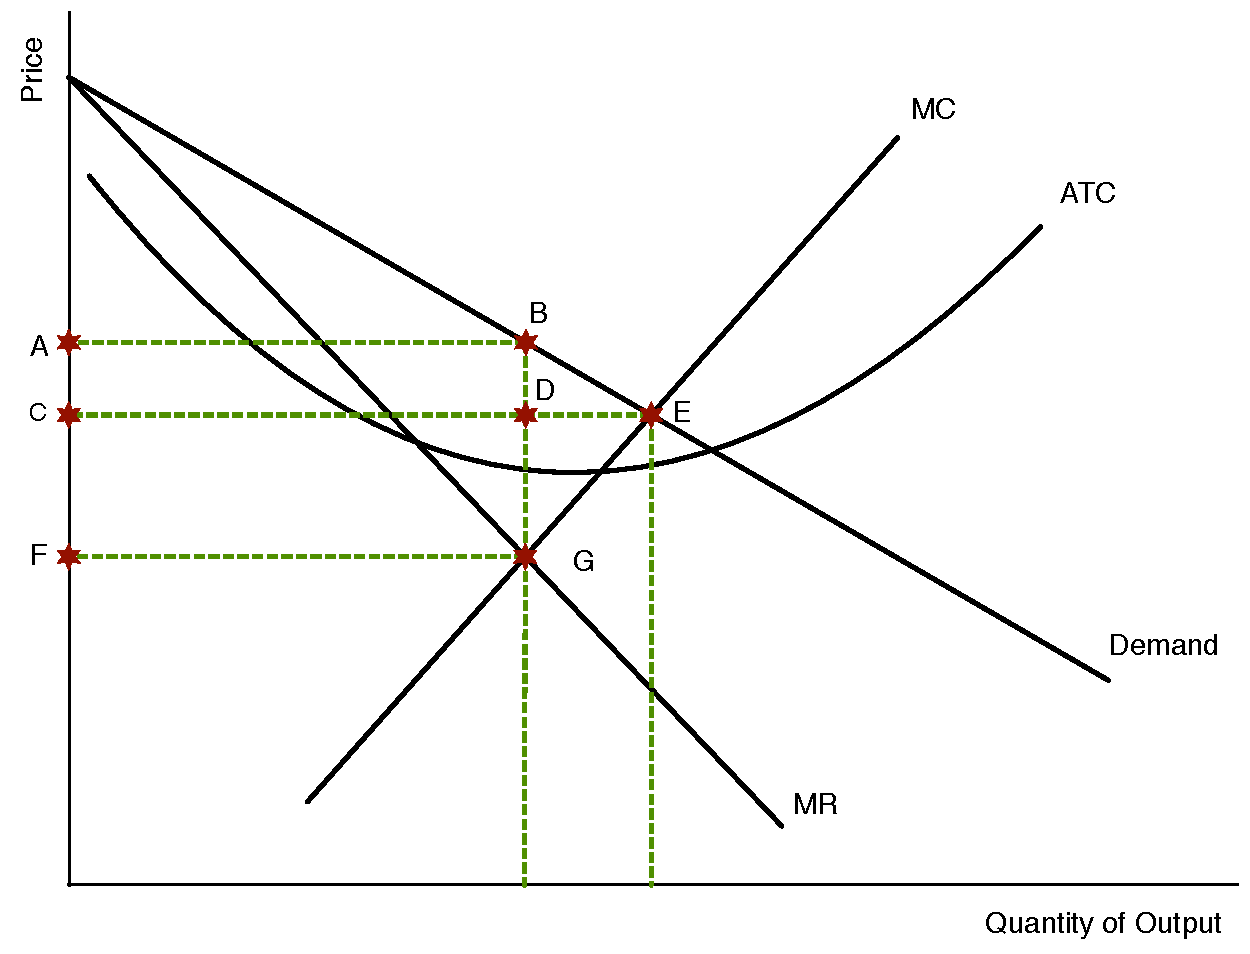
\includegraphics[scale=.4]{Exam2_MC10.pdf}
	\caption{Monopolist Environment}
	\label{MC10}
\end{figure}
	
	\question \label{q4} Charging price \blank maximizes the monopolist's profit, while total surplus is maximized at price \blank.
	
	\begin{choices}
		\choice C; A
		\choice F; C
		\CorrectChoice  A; C
		\choice A; F
		\choice None of the above.
	\end{choices}
	
	\begin{solution}
		The monopolist produces at $Q$ where $MR=MC$. Trace up to the demand curve to find the price ($A$). Efficient point is where $P=MC$, i.e., where demand meets the marginal cost curve at point $E$. Trace across to find the price ($C$).
	\end{solution}
	
\newpage
	
	\question \label{q5} Which of the following distances represents the mark-up over marginal cost at the profit maximizing quantity?
	
	\begin{choices}
		\choice Distance AC
		\choice Distance DE
		\choice Distance CF
		\CorrectChoice Distance BG
		\choice None of the above.
	\end{choices}
	
	\begin{solution}
		$Q^*$ is where $MR=MC$. The mark-up, $\mu$ is the difference between the price and $MC$ (distance between the demand and marginal cost curve at $Q^*$).
	\end{solution}

	
	\question Firms in monopolistically competitive markets are similar to monopolies in that they both \blank and are similar to firms in perfectly competitive markets in that they both \blank.
	
	\begin{choices}
		\choice are price makers; produce at the efficient quantity
		\choice make positive profits in the short and long run; produce at the efficient scale in the long run
		\CorrectChoice charge a price above the marginal cost; can freely enter and exit the market
		\choice are in markets with barriers to entry; make zero economic profit in the long run
	\end{choices}
	
	\begin{solution}
		See class notes.
	\end{solution}
	
	\question A monopolistically competitive firm will increase its production if
	
	\begin{choices}
		\CorrectChoice marginal revenue is greater than marginal cost.
		\choice marginal revenue is greater than average total cost.
		\choice price is greater than average total cost.
		\choice price is greater than marginal cost.
	\end{choices}
	
		\begin{solution}
			See class notes and Homework 3.
		\end{solution}

	
		
\uplevel{Use the following information to answer questions \ref{q8} - \ref{q9}. Suppose we are studying a market where each unit bought and sold incurs an external cost of \$3 on society. However, the sale of this good also provides an external benefit of \$5 per unit.}

	
\question \label{q8} In the absence of government intervention, the market will provide an amount

\begin{choices}
	\CorrectChoice smaller than the efficient output level.
	\choice greater than the efficient output level.
	\choice equal to the efficient output level.
	\choice Not enough information given.
\end{choices}

\begin{solution}
	$EB > EC$, so the market will underprovide the good.
\end{solution}

\question \label{q9} In order to induce the market to produce the efficient quantity, the government could 

\begin{choices}
	\choice impose a \$2 per-unit tax on sellers.
	\choice provide a \$5 per-unit subsidy to buyers. 
	\choice impose a \$3 per-unit tax on buyers.
	\CorrectChoice provide a \$2 per-unit subisdy to buyers.
	\choice None of the above.
\end{choices}

\begin{solution}
	EB - EC = \$2. Should provide a subsidy so more of the good is produced.
\end{solution}
	
	\question Refer to Figure \ref{MC2}.


\begin{figure}[H]
	\centering
	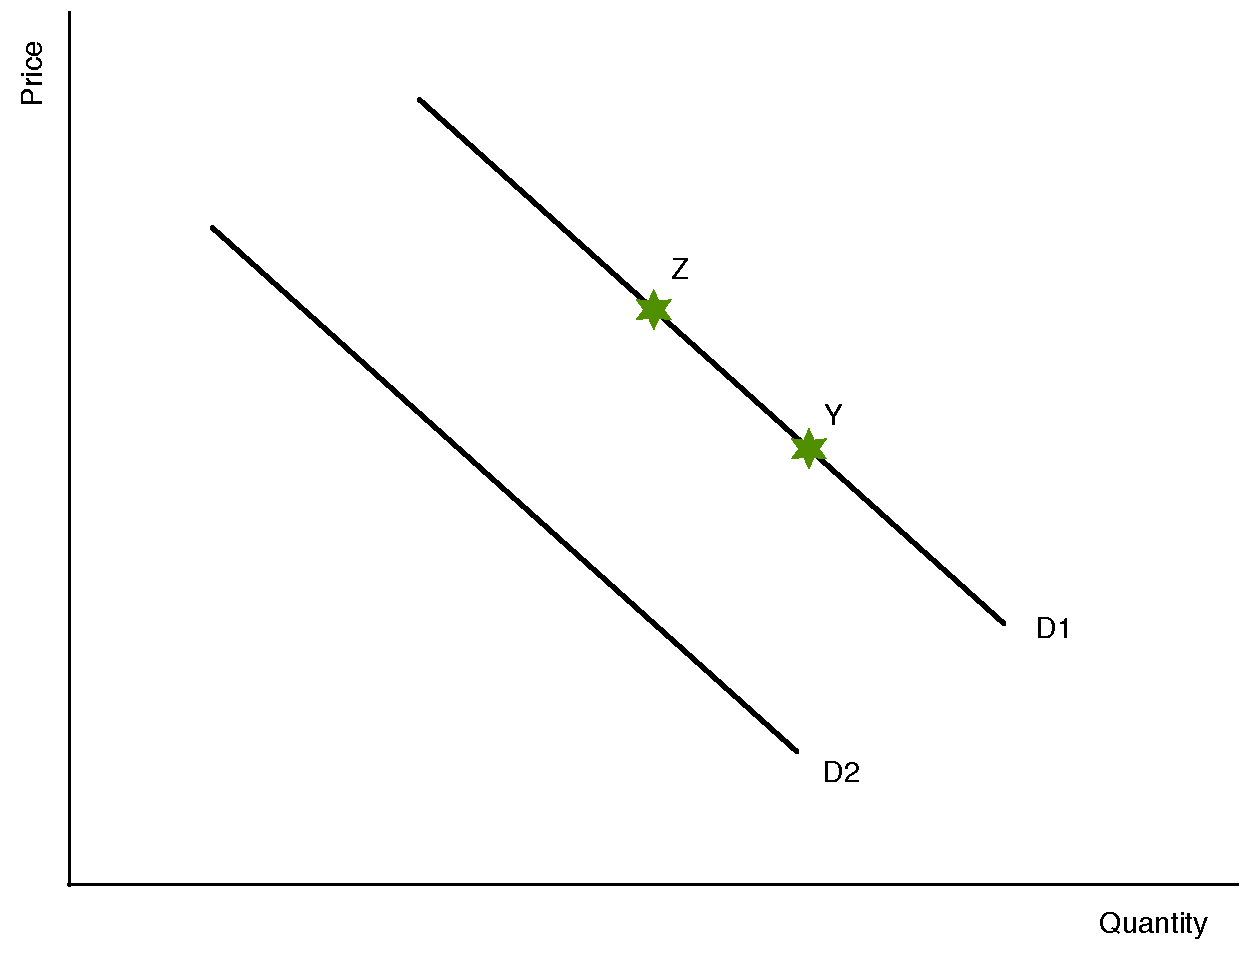
\includegraphics[scale=.35]{Exam1_MC2.pdf}
	\caption{Demand for Shrimp}
	\label{MC2}
\end{figure}
	
	All else equal, a decrease in the income of buyers who consider shrimp to be an inferior good would cause a move from
	
	\begin{choices}
		\CorrectChoice D2 to D1.
		\choice Y to Z.
		\choice Z to Y.
		\choice D1 to D2.
	\end{choices}
	
	\begin{solution}
		A decrease in income will increase demand for an inferior good.
	\end{solution}
	
	
	\question A non-congested toll road is an example of a \blank because it is \blank.
	
	\begin{choices}
		\CorrectChoice club good; excludable and non-rival
		\choice common resource; non-excludable and rival
		\choice private good; excludable and rival
		\choice public good; non-excludable and non-rival
	\end{choices}
	
	\begin{solution}
		Non-congested - non-rival. Toll road - excludable.
	\end{solution}
	

	\question The market for Twist is currently at equilibrium and the price of the drink is \$1.00 per can. Under pressure from consumers, the government imposes a price ceiling of \$1.25 per can, leading to \blank in producer surplus and \blank in total surplus.
	
	\begin{choices}
		\choice no change; an increase
		\choice an increase; an increase
		\choice a decrease; a decrease
		\choice a decrease; no change
		\CorrectChoice no change; no change
	\end{choices}
	
	\begin{solution}
		The price ceiling is above equilibrium market price, so it will be non-binding.
	\end{solution}


\newpage
	
\uplevel{Use Table \ref{MC8}, which shows the number of hours it takes Katie and Megan to harvest one apple or pear, and the information below to answer questions \ref{q12} - \ref{q14}.}
	
\begin{table}[H]
	\caption{Number of hours to harvest one:}
	\centering
	\begin{tabular}{ c|c|c} 
		
		   & Apple & Pear \\
		\hline
		Katie & 3 & 5 \\
		Megan & 2 & 4 \\
	\end{tabular}
	\label{MC8}
\end{table}

\begin{solution}
	Katie. 1/3 apple : 1/5 pear $\Rightarrow$ 1 pear : 1.67 apples.\\
	Megan. 1/2 apple : 1/4 pear $\Rightarrow$ 1 pear : 2 apples. \\
	Terms of trade for both to be better off: 1 pear : $x$ apples, where $1.67 < x < 2$. \\
	If $x<1.67$, Katie is worse off and Megan is better off. \\
	If $x>2$, Megan is worse off and Katie is better off.\\
\end{solution}

The parties decide to trade and the following terms are proposed:

\begin{enumerate}[i.]
	\item 200 apples per 400 pears \begin{solution}1 pear : .5 apples - Katie worse off, Megan better off \end{solution}
	\item 100 apples per 400 pears \begin{solution}1 pear : .25 apples - Katie worse off, Megan better off \end{solution}
	\item 55 pears per 100 apples \begin{solution}1 pear : 1.82 apples - Both better off \end{solution}
	\item 100 pears per 400 apples \begin{solution}1 pear : 4 apples - Megan worse off, Katie better off \end{solution}
\end{enumerate}


\question \label{q12} Given this information, it follows that 
	
	\begin{choices}
		\choice Katie has an absolute advantage in the production of apples, while Megan has an absolute advantage in the production of pears.
		\choice Katie has an absolute advantage in the production of both apples and pears.
		\choice Megan has an absolute advantage in the production of apples, while Katie has an absolute advantage in the production of pears.
		\CorrectChoice Megan has an absolute advantage in the production of both apples and pears.
	\end{choices}
	
	\begin{solution}
		It takes Megan less hours to produce one of either good than Katie.
	\end{solution}
	
\question \label{q13} Of the terms of trade proposed, how many would make Katie better off, but would make Megan worse off than without trade?

\begin{choices}
	\choice 0
	\CorrectChoice 1
	\choice 2
	\choice 3
	\choice 4
\end{choices}

\begin{solution}
	Katie is better off as long as she gets more than 1.67 apples per pear, while Megan is worse off if she gives up more than 2 apples per pear. (iv) would make Katie better off (receives 4 apples per pear) but would make Megan worse off (gives up 4 apples per pear).
\end{solution}
	
\question \label{q14} Of the terms of trades proposed, how many would make both parties better off than without trade?
	
	\begin{choices}
		\choice 0
		\CorrectChoice 1
		\choice 2
		\choice 3
		\choice 4
	\end{choices}
	
	\begin{solution}
		Only (iii) would make both parties better off.
	\end{solution}
	
\newpage
		
\question Chocolate chip cookies and milk are complements. If the demand for chocolate chip cookies increases, then the equilibrium price of milk will \blank and the equilibrium quantity will \blank.
	
	\begin{choices}
		\choice increase; decrease
		\choice decrease; increase
		\choice increase; increase
		\CorrectChoice decrease; decrease
	\end{choices}
	
	\begin{solution}
		An increase in demand for cookies will increase the price of cookies. This will decrease demand for milk (since the price of a complement went up), so the equilibrium price and quantity of milk will both decrease.
	\end{solution}
	
	\question If chocolate chip cookies and oatmeal raisin cookies are substitutes, the cross-price elasticity of demand between the goods is
	
	\begin{choices}
		\choice negative.
		\CorrectChoice positive.
		\choice zero.
		\choice impossible to discern without more information.
	\end{choices}
	
	\begin{solution}
		The cross-price elasticity of substitutes is positive.
	\end{solution}
	

	\question Refer to Figure \ref{MC16}, which shows the market for laptop computers.
	
\begin{figure}[H]
	\centering
	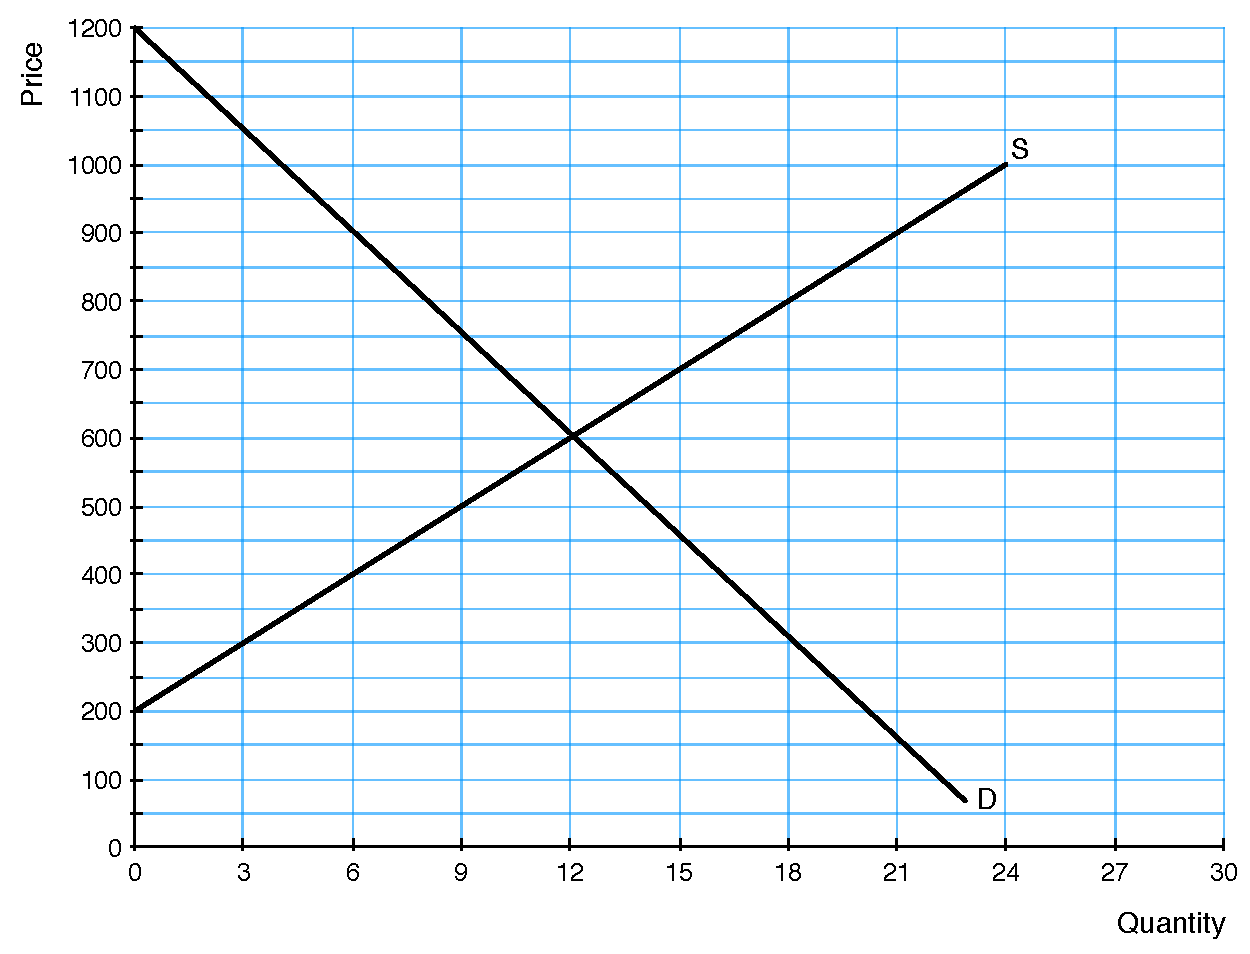
\includegraphics[scale=.45]{Exam1_MC16.pdf}
	\caption{Market for Laptops}
	\label{MC16}
\end{figure}

If a tax of \$500 is imposed on buyers, then the share of the tax paid by consumers is
	
	\begin{choices}
		\choice \$200.
		\CorrectChoice \$300.
		\choice \$500.
		\choice \$900.
	\end{choices}
	
	\begin{solution}
		Tax wedge of \$500 $\Rightarrow P_B = 900$, $P_S = \$400$. Price before tax = \$600, so buyers bear \$300 of the burden.
	\end{solution}
	
\newpage
	
	\question Table \ref{MC17} shows the quantity supplied and demanded at certain prices.

	
	\begin{table}[H]
		\caption{Prices and Quantities}
		\centering
		\begin{tabular}{ c|c|c} 
			
			Price & $Q_d$ & $Q_s$ \\
			\hline
			\$10 & 50 & 30 \\
			\$12 & 45 & 35 \\
			\$14 & 40 & 40 \\
			\$16 & 35 & 45 \\
			\$18 & 30 & 50 \\
		\end{tabular}
		\label{MC17}
	\end{table}
	
	If the price in the market were \$16, there would be
	
	\begin{choices}
		\choice a shortage of 10 units.
		\choice a surplus of 45 units.
		\choice a shortage of 35 units.
		\CorrectChoice a surplus of 10 units.
	\end{choices}
	
	\begin{solution}
		At a price of 16, $Q_d = 35 < Q_s = 45$. Surplus of 10 units.
	\end{solution}
		
	
	\question The opportunity cost of attending college does \textbf{not} include
	
	\begin{choices}
		\choice the potential salary you could earn by quitting school and working now.
		\choice the costs of room and board, books, and class materials.
		\CorrectChoice the potential salary you could earn after finishing your degree.
		\choice the psychological costs of stress and lack of sleep.
	\end{choices}
	
	\begin{solution}
		(c) is not part of the opportunity cost of going to college, since you are not giving up this higher future salary by attending.
	\end{solution}
	
	\question As individuals lose their jobs, they buy fewer romance novels. Which of the following might be the income elasticity of demand for romance novels?
	
	\begin{choices}
		\choice $-1.32$
		\choice $-.30$
		\CorrectChoice $.54$
		\choice Either (a) or (b)
	\end{choices}
	
	\begin{solution}
		Less income leads to a decrease in $Q_d$, so romance novels are normal goods. $\varepsilon_d^I > 0$.
	\end{solution}
	
	\question A firm currently produces 1,000 units of output with an average total cost of \$10.10. The firm has fixed costs of \$5,000. If the firm were to produce 1,001 units, its total variable costs would be \$5,400. What is the marginal cost to the firm of producing 1,001 units?
		
		\begin{choices}
			\choice \$4,700
			\CorrectChoice \$300
			\choice \$5,100
			\choice \$400
		\end{choices}
		
		\begin{solution}
			At Q=1,000, TC = 10.10$\times$ 1000 = 10,100. At Q=1,001, TC = 5,400 + 5,000 = 10,400. $MC = 10,400-10,100 = 300$.
		\end{solution}
		
\newpage
	
	\question The United States currently produces guns and butter. Table \ref{MC22} shows possible combinations of the two goods the US can produce in a given week (in thousands). 
	
	\begin{table}[h!]
		\caption{Weekly Production of Guns and Butter}
		\centering
		\begin{tabular}{ c|c} 
			
			Guns & Butter (lbs) \\
			\hline
			100 & 800 \\
			200 & $x$  \\
			300 & 500 \\
		\end{tabular}
		\label{MC22}
	\end{table}
	
	If resources in the US are specialized such that some are better suited to producing guns and others are better suited for butter production, then a possible value for $x$ might be
	
	\begin{choices}
		\choice 650.
		\choice 550.
		\choice 600.
		\CorrectChoice 700.
	\end{choices}
	
	\begin{solution}
		Specialization of resources leads to increasing opportunity costs. OC of moving from 100 to 200 guns < OC of moving from 200 to 300 guns $\Rightarrow$ $  650 < x < 800$.
	\end{solution}
	
	\question A per-unit tax of \$6 is imposed by the government. Use Table \ref{MC27} to answer the question below.
	
	\begin{table}[h!]
		\caption{Unit Taxes}
		\centering
		\begin{tabular}{ c|c|c} 
			
			& Price with no tax & Price with \$6/unit tax on sellers \\
			\hline
			Price paid by buyers & \$55 & ? \\
			Price paid by sellers & \$55 & \$53.50  \\
		\end{tabular}
		\label{MC27}
	\end{table}

Because of this tax, buyers are paying \blank per unit and sellers are receiving \blank per unit.

	\begin{choices}
		\choice \$1.50 more; \$4.50 less
		\choice \$3 less; \$3 more
		\CorrectChoice \$4.50 more; \$1.50 less
		\choice \$2 more; \$4 less
	\end{choices}
	
	\begin{solution}
		$P_B = P_S + tax = 53.50 + 6 = \$59.50$. Buyers paying 4.50 more per unit, sellers receiving 1.50 less.
	\end{solution}
	
	\question The property of production functions whereby the marginal product of an input decreases as the number of inputs increases is called 
	
	
	\begin{choices}
		\choice increasing returns to inputs.
		\choice diseconomies of scale.
		\CorrectChoice diminishing marginal product.
		\choice economies of scale.
		\choice constant returns to scale.
	\end{choices}
	
	\begin{solution}
		See class notes. 
	\end{solution}
	
\newpage


		
\question Suppose that the price of wine, a substitute for beer, decreases. As a result, the equilibrium price of beer \blank and total surplus in the beer market \blank. 

\begin{choices}
	\choice increases; increases
	\choice increases; decreases
	\CorrectChoice decreases; decreases
	\choice decreases; increases
\end{choices}

\begin{solution}
	Demand for beer will decrease, which will decrease the equilibrium price and quantity of beer. This will decrease total surplus.
\end{solution}


\question Stella's Nail Salon provided 100,000 haircuts last year with a total variable cost of \$800,000. If the average fixed cost of the haircuts was \$5, what was the company's average total cost of the haircuts last year?


\begin{choices}
	\choice Exactly \$8
	\CorrectChoice More than \$10
	\choice Less than \$8
	\choice More than \$8, but less than \$10
\end{choices}

\begin{solution}
	$ATC = AFC + AVC = \$5 + 800,000/100,000 = \$13$.
\end{solution}
	
	\question Matthew is trying to determine how many sticks of RAM he should buy for his computer. Each additional stick increases the speed of his computer by 50\%. On a typical day, he would be willing to pay \$100 for each 50\% increase in computing power. The total costs of acquiring and installing each stick of RAM are detailed in Table \ref{MC30}. 
	
	\begin{table}[H]
		\caption{Total Costs of RAM}
		\centering
		\begin{tabular}{c|c} 
			
			 Sticks of RAM &  Total Cost\\
			\hline
			1 & \$40 \\
			2 & \$100  \\
			3 & \$175 \\
			4 & \$265 \\
			5 & \$370 
		\end{tabular}
		\label{MC30}
	\end{table}

	How many sticks of RAM should Matthew purchase?

	\begin{choices}
		\choice 1
		\choice 2
		\choice 3
		\CorrectChoice 4
		\choice 5
	\end{choices}
	
	\begin{solution}
		Matthew should buy the next stick of RAM as long as $MB \ge MC$. Find the marginal cost from the total cost column. $MC$ of 1st stick = \$40, 2nd stick = \$60, 3rd stick = \$75, 4th stick = \$90, 5th stick = \$105.  $MB = \$100$ per stick, so Matt should buy 4 sticks of RAM.
	\end{solution}
	
\newpage
	
		\question Refer to Table \ref{wtp}, which gives the costs to sell 1 lb of cauliflower for four individuals.
		
		\begin{table}[H]
			\caption{Costs for 1 lb Cauliflower}
			\label{wtp}
			\centering
			\begin{tabular}{  c|c    }    
				
				Seller   & Cost \\
				\hline
				Jasmine & \$4.00 \\
				Tyler & \$2.50 \\
				Deepak & \$3.00 \\
				Sarah & \$.50 \\
			\end{tabular}
			
		\end{table} 
		
		Suppose the price of cauliflower increases from \$2.00 to \$3.50. The change in total producer surplus that is due to sellers entering or exiting the market because of the price change is
		
		\begin{choices}
			\choice \$1.00.
			\choice \$3.00.
			\choice \$4.50.
			\CorrectChoice \$1.50.
		\end{choices}
		
		\begin{solution}
			Sell as long as $SC > P$. At $P_0$ = \$2, only Sarah was selling cauliflower and realized $PS_0 = (\$2 - .50) = \$1.50$. At $P_1$ = \$3.50, Sarah, Tyler, and Deepak are willing to sell and realize surplus of $PS_1 = (3.50 - .50) + (3.50 - 2.50) + (3.50 - 3) = \$4.5$. Increase in surplus to old seller: \$1.50. Increase in surplus due to new sellers: \$1.50.
		\end{solution}
	

	
	\question Jen's Shop is a firm in a perfectly competitive market and has the cost structure shown in Figure \ref{MC28}.
	
	\begin{figure}[H]
		\centering
		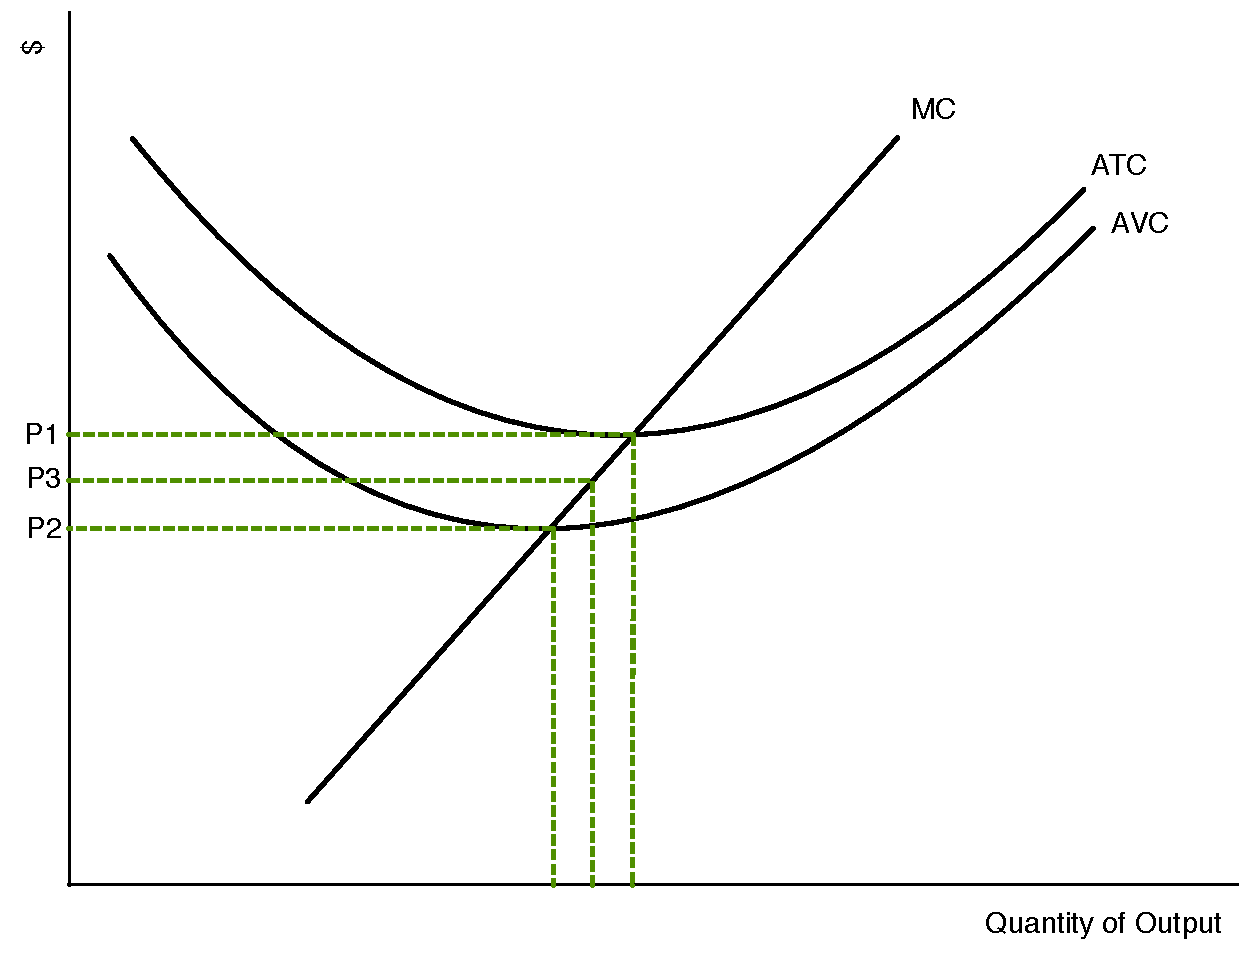
\includegraphics[scale=.37]{Exam1_MC27.pdf}
		\caption{Jen's Shop}
		\label{MC28}
	\end{figure}
	
	If the market price were strictly between $P1$ and $P3$, then the firm would \blank in the short run and make \blank profit.
	
	\begin{choices}
		\CorrectChoice operate; negative
		\choice operate; zero
		\choice shutdown; negative
		\choice shutdown; zero
	\end{choices}
	
	\begin{solution}
		$P$ is along part of $MC$ curve above $AVC$, so should operate, but $P < ATC$ and so the firm would make a loss.
	\end{solution}
	
\end{questions}

\newpage

\section*{Short Answer}

For this section, make sure to write legibly and box final answers. \textbf{Show your work!} This can be done within the section or \textit{clearly} labeled on the scratch paper provided.

\begin{questions}


	\question Table \ref{SA2} shows the willingness to pay and costs of six buyers and sellers in the market for headphones. Each buyer would like to purchase one pair and each seller has one pair to sell. 
	
\begin{table}[H]
		\caption{WTP and Seller Costs for Headphones}
		\centering
		\begin{tabular}{c|c} 
			
			WTP   & Seller Costs \\
			\hline
			\$175 & \$80 \\
			\$100 & \$140 \\
			\$120 & \$120 \\
			\$200 & \$130 \\
			\$140 & \$180 \\
			\$160 & \$155\\
		\end{tabular}
		\label{SA2}
\end{table}

Use the table to answer the following questions.

\begin{solution}
	\begin{table}[H]
		\caption{WTP and Seller Costs for Headphones}
		\centering
		\begin{tabular}{c|c|c|c|c} 
			
			WTP   & SC  & TS = WTP - SC  &  SC$_{tax}$ = SC + tax & TS$_{tax}$ = WTP - SC$_{tax}$ + tax \\
			\hline
			\$200 & \$80  & \$120 & \$135 & \$120 \\
			\$175 & \$120 & \$55 & \$175 & \$55 \\
			\$160 & \$130 & \$30 & \$185 & --- \\
			\$140 & \$140 & \$0 &  \$195 & --- \\
			\$120 & \$155  & --- & \$210 & --- \\
			\$100 & \$180 & --- & \$235 & --- \\
		\end{tabular}
	\end{table}
\end{solution}
	
	
	\begin{parts}
		\part[2] If the market price is currently \$120, is there a shortage or a surplus? Explain why. What do you expect will happen to the market price?
		 
		\begin{solution}[.5in]
			At $P = 120$, $Q_d = 5$ and $Q_s = 2$. This would lead to a shortage and the market price would increase.
		\end{solution}
		
		\part[2] What is the market equilibrium price and quantity in this market? 
		
		\begin{solution}[.5in]
			Order WTP from highest to lowest and seller costs from lowest to highest. Equilibrium is where they meet. ($P^*,Q^*) = (\$140,4)$.
		\end{solution}
		
		\part[2] At the market equilibrium, what is the total surplus realized? 
		
		\begin{solution}[.5in]
			$TS = (200 - 80) + (175 - 120) + (160 - 130) + (140 - 140) = \$205$.
		\end{solution}
		
		\part[3] Suppose the government imposes a per-unit tax of \$55 on sellers of headphones. What will be the price buyers pay, the price sellers receive, and the quantity exchanged in the market as a result of this tax? 
		
		\begin{solution}[.5in]
			The tax will increase seller costs by \$55 each. Find where WTP and SC meet after this. $Q_T = 2$. $P_B = \$175$, $P_S = \$120$.
		\end{solution}
		
		\part[2] Who bears most of the tax burden, buyers or sellers? What does this tell you about the relatively elasticity of supply and demand? 
		
		\begin{solution}[.75in]
			Sellers bear $(140 - 120) = \$20$ of the tax, while buyers bear $(175 - 140) = \$35$ of the tax. Buyers bear more of the burden because demand is relatively more inelastic than supply.
		\end{solution}
		
		\part[2] What is the tax revenue generated from this tax and the deadweight loss incurred as a result?
		
		\begin{solution}[.5in]
			Tax revenue = \$55 $\times$ 2 = \$110. Easy way to find DWL = unrealized gains from trade $= (160 - 130) + (140 - 140) = \$30$ (lost surplus from third and fourth transactions that were taking place without the tax).
		\end{solution}
	\end{parts}
	
	
	\question A firm is currently in a market with the conditions outlined in Table \ref{SA3}. The firm has fixed costs of \$1,500 per day.
	
\begin{table}[H]
	\caption{Market Environment}
	\centering
	\begin{tabular}{c|c|c|c|c} 
		
		Quantity/day   & Total Revenue &  Marginal Cost & Variable Costs & Total Costs\\
		\hline
		1 & \$600 &  \$1,000 & \dd{1000} & \dd{2500}  \\
		2 & \$1,200 & \$400 & \dd{1400}  & \dd{2900} \\
		3 & \$1,800 & \$500 & \dd{1900}  & \dd{3400}  \\
		4 & \$2,400 & \$600 & \dd{2500} & \dd{4000} \\
		5  & \$3,000 & \$800 & \dd{3300}  & \dd{4800} \\
	\end{tabular}
	\label{SA3}
\end{table}

	Use this information to answer the following questions.
	
	\begin{parts}
		\part[2] What type of market environment is this firm in? Explain why. 
		
		\begin{solution}[.5in]
			The firm is in a perfectly competitive market since $P = MR = \$600$.
		\end{solution}
		
		\part[2] Fill in the column labeled ``Variable Costs.'' 
		
		\begin{solution}
			See Homework 2, \#29 for an example of this.
		\end{solution}
		
		\part[2] Fill in the column labeled ``Total Costs.'' 
		
		\part[4] What level of production should the firm operate at? Explain why.
		
		\begin{solution}[.75in]
			The firm should operate at $Q^* = 0$ (shutdown) because $VC > TR$ at the quantity where $MR = MC$ ($Q=4$).
		\end{solution}
		
		\part[2] What will be the firm's profits per day at this production level?
		
		\begin{solution}[.75in]
			$\Pi = -\$1,500$ (fixed costs).
		\end{solution}
	\end{parts}
	
\end{questions}

\hrulefill
\begin{center} 
	\textbf{END OF EXAM}
\end{center}

\newpage

\centering

\section*{SCRATCH SHEET}



\end{document}